\section{Topic Modelling}
Topic Modelling is an unsupervised machine learning and statistical modelling approach which aims to discover the abstract "topics" in a collection of documents, referred to as the corpus. This can be used to find hidden semantic structures in a document. This works by looking at how often words appear in the corpus and trying to create topics made of words which are related to each other. For example an article about dogs would be more likely to have words such as "dog" and "bone", and thus the topic model would most likely group those two words together into a topic. 

There are many approaches to topic modelling, one of the foremost examples is Latent Dirichlet Allocation, which aims to reverse engineer the topics by assuming the text was created from K topics and all words directly relate to one of the K topics. There are other forms of clustering algorithm which can be applied to words, such as the K Means clustering algorithm. 

\subsection{Latent Dirichlet Allocation}
Latent Dirichlet Allocation (LDA) is an unsupervised learning model which aims to collate words into K topics. When performing LDA, the text to be clustered is split into a series of documents, each composed of a bag of words where the order of the words doesn't matter. Most of the time, this will required pre-processing to remove words which do not contribute to the topics present in the work such as `the`, `is`,  and `a`. 

\noindent The algorithm works by making the assumption that the document was made by first picking K topics, and then picking words around each topic. Then, the algorithm reverse engineers this process, by first assuming that there are K topics in the document. The K topics are then distributed across each document, such that each word in each document is assigned a topic. The topic distribution across the whole text is performed according to a matrix, $\alpha$,  where each row is a document, and each column is a topic, and the $i_{th}$ row and $j_{th}$ column represent the likelihood of the topic j being in document i. This distribution can be symmetric i.e. each topic is equally likely across a document, or it can be asymmetric, where certain topics are favoured.

\noindent After assigning the topics across the document, and to each of the words, the topics are reassigned for each word. This is done by changing the topic for each word individually and in order. The new topic for each word is based on two factors, firstly what topics already exist in that document, and the number of times each topic was assigned to that word in all of the other documents. The word is then assigned a new topic probabilistically taking these two factors into consideration.

\noindent This process is repeated several times across all of the words for all of the documents, until the topic distribution is done. A visual example of the LDA model is shown in Figure \ref{fig:ldafigure}. In this, M denotes the number of documents,
N represents the number of words in each document such that document i has $N_{i} words)$, $\alpha$ is the topic distribution across topics, $\beta$ is the word distribution across topics, $\theta$ is the topic distribution for each document M, $\phi$ is the word distribution for each topic K. Z represents the topic for the \textit{n}-th word in the document m, and w represents each specific word. It should be noted that W is the only observable variable in the system, and all others are latent. In the original paper, the topic-word distribution can be modelled using a sparse Dirichlet prior, as it would be thought that the probability distribution of words in a topic will be skewed, such that only a small number of words have high probabilities. 

\begin{figure}
	\centering
		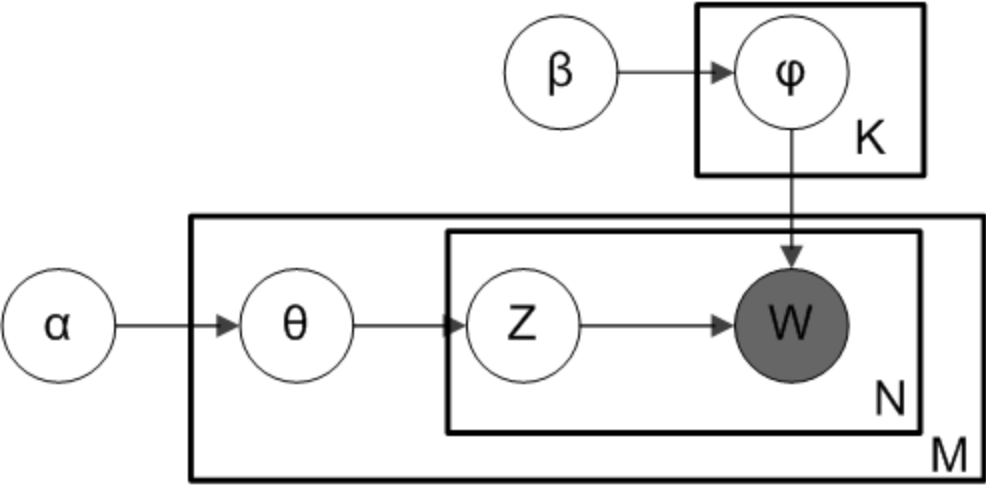
\includegraphics[width=0.6\textwidth]{images/LDA.png}
	\caption{A Graphical Plate representation of (smoothed) LDA (image from \cite{LDA})}
	\label{fig:ldafigure}
\end{figure}


LDA has been used widely for topic modelling across many fields.  This has also been used in stock market predictions by attempting to mine many different kinds of data to used as prediction. This includes seeing if anything from social media data \cite{nguyen2015sentiment}, to topics in financial news \cite{feuerriegel2016analysis} affect stock prices .This is similar to the goal of this dissertation, and thus this was deemed a suitable metric to use for this purpose. 
 
 \subsection{Term Frequency-Inverse Document Frequency}
 Tf-idf is a well known numeric statistic used to calculate the importance of a word to a document in a collection or corpus. It works on the basis of creating a weighting for each word, based on the product of the term frequency and the inverse document frequency. The term frequency is the count of how many times each word appeared in the document. The inverse document frequency aims to measure how much information a word provides to the document, i.e. if the word appears extremely often (e.g. the word `the`), it would attain a lower idf score, and vice versa. It is calculated by taking the logarithm of the inverse of the fraction of documents which contain that word. This is shown below:
 
 \begin{center}
 	$tf(t,d) = f_{t,d}$\\
 	$idf(t, D) = log\frac{N}{\{d \in D : t \in D\}}$
 \end{center}
 
 Tf-idf is used extensively in text mining, as it shows the most important words of a corpus, this is used extensively, from paper recommender systems \cite{beel2016paper}, search engines \cite{xu2014pos}, and digital libraries \cite{philip2014application} alongside other uses. This has also been used extensively for predicting stock prices, as part of a wider prediction using sentiment analysis model. 
 
 
\subsection{K Means Clustering}
Another methodology of grouping objects together is to use a clustering algorithm such as the K Means algorithm. This is a simple algorithm, which randomly places the centres of K clusters within the data, and then each data point is assigned to the nearest cluster, and a total cost is calculated based on a distance metric between each cluster centre and all of the points assigned to the centre. The cluster centres are then moved closer to the `centre` of the points assigned to that cluster, then if necessary, the points are reassigned to the nearest cluster and the cost re-calculated. The algorithm will finish when the assignments do not change (within a tolerance). It should be noted that this algorithm is heavily dependant on the starting positions of the cluster centres, and is not guaranteed to find the optimal solution. As such it remains an computationally NP hard problem. 

The K Means clustering algorithm only works with numerical data in n dimensions as it needs to quantify the distance between two points. Thus if K means were used to cluster words, the words would have to be transformed into a numeric representation. A naive solution would be to just use the ASCII values of the words. However to perform clustering effectively based on the meaning of the words and relevance to the text as a whole, the numerical value would have preserve any underlying relationship between the words and the document overall, which isn't possible if ASCII was the one which was used. Thus, Tf-idf would be such a measure, as it weights the importance of a word to a text, and the frequency of usage. 

This combined method of using TFIDF with K Means is widely used. It has been used for summarisation of document spaces \cite{khan2019extractive}, for classification \cite{buana2012combination}, and specifically for topic detection \cite{6066301}. Thus, this was considered a suitable approach for topic classification.

\subsection{Mahalanobis distance}
One of the biggest challenges with using K Means for word clustering is the use of the Euclidean distance for measuring distance. The Mahalanobis distance offers another methodology for calculating the distance between 2 points. It was originally designed to calculate the distance between a point and a distribution, but can be used to calculate the distance between 2 points in multi-variate space. The advantage of using the Mahalanobis distance is that it takes into consideration the correlation in the underlying data, so if used with the K Means clustering, the variance covariance matrix of the data can be used. The Mahalanobis distance would mainly be used after the cluster has been fitted (since the final variance covariance matrix is required), to calculate the distance between a new point and the centres of the clusters, as below, where $X_{c}$ represents the data the cluster is made with, $x_{i}$ represents a point and $\bar{x_{i}}$ represents a cluster centroid.  

\begin{center}
	Covariance Matrix:
	$C_{x} = \frac{1}{n - 1} (X_{c}) ^T (X_{c})$
	
	Mahalanobis Distance:
	$MD_{i} = \sqrt{(x_{i}  -  \bar{ x  } ) C_{x}^{-1} ( x_{i}   - \bar{ x  }  )^T    }  $
\end{center}

The Mahalanobis distance has been used with clustering algorithms such as k-means \cite{melnykov2014k} \cite{cerioli2005k}, and is frequently used in distributions of clusters which are either elliptical \cite{mitchell1985mahalanobis} or non normal distributions \cite{warren2011use}. Since the distribution of points around the k means clusters is likely to be unknown with using a Tf-Idf vectorizer, this was seen as a suitable metric to use for evaluating the clusters the algorithm would create.